\chapter{कोशिका विभेदन: कंकाल पेशी कोशिका}\label{ch:b2:cell-differentiation}

आपकी जाँघ की पेशी का एक तंतु तीस सेंटीमीटर लंबी एक ही कोशिका है, जिसमें
सैकड़ों केंद्रक हैं और जो सिरे से सिरे तक इतनी नियमित संकुचनशील छड़ों से
भरी है कि सूक्ष्मदर्शी के नीचे धारीदार दिखती है। उसका आरंभ साधारण दिखती
कोशिकाओं के एक गुच्छे से हुआ था जो किसी कायखंड से रेंगकर निकलीं, गुणित
हुईं, विभाजित होना बंद किया, पंक्ति में लगीं, संलयित हुईं, और कई सौ ऐसे
जीन चालू कर दिए जो उन्होंने पहले कभी काम में नहीं लिए थे। शरीर की हर
कोशिका का जीनोम वही है; और \omterm{def:b2:cell-differentiation:myogenesis}{पेशी तंतु}
वह है जो वही जीनोम तब करता है जब कोई एक विशेष \omterm{prop:b2:cell-differentiation:transcriptional}{अनुलेखन कारक}
चालू कर दिया जाए। यह अध्याय कंकाल पेशी कोशिका को
\emph{\omterm{def:b2:cell-differentiation:differentiation}{विभेदन}} का हल किया हुआ उदाहरण मानता है --- यानी यह कि कोई कोशिका
कोई विशिष्ट पहचान कैसे पाती और बनाए रखती है --- और पेशी कोशिका अच्छा
उदाहरण इसलिए है कि उसका प्रमुख स्विच ज्ञात है, उसके चरण किसी तश्तरी में
देखे जा सकते हैं, और तैयार कोशिका ऐसी मशीन है जिसके पुर्ज़े दिखते हैं।

\section{विभेदन क्या है}

\begin{definition}[विभेदन, निर्धारण, शक्तता]\label{def:b2:cell-differentiation:differentiation}
\index{विभेदन}\index{निर्धारण (कोशिका)}\index{स्तंभ कोशिका}\index{शक्तता}
कोई कोशिका \emph{विभेदित} तब है जब वह किसी एक कोशिका-प्रकार के जीनों का
--- और इसलिए प्रोटीनों, आकार तथा कार्य का --- स्थिर प्रतिरूप
अभिव्यक्त करे। वह \emph{निर्धारित} (या प्रतिबद्ध) तब है जब उसकी नियति
तय हो चुकी हो यद्यपि उसका विभेदन अभी आरंभ न हुआ हो: कोई \omterm{def:b2:cell-differentiation:myogenesis}{पेशीकोरक}
किसी तंतुकोरक जैसा दिखता है पर बनाएगा केवल पेशी। \emph{शक्तता}
उन प्रकारों की परास है जो कोई कोशिका अब भी दे सकती है: \emph{पूर्णशक्त}
(युग्मनज और पहली कोरकखंड, जो \omterm{def:b2:mammal-reproduction:placenta}{अपरा} समेत सब कुछ बनाती हैं),
\emph{बहुशक्त} (\omterm{def:b2:mammal-reproduction:implantation}{अंतःकोशिका पिंड}, जो शरीर का
हर ऊतक बनाता है), \emph{अनेकशक्त} (रक्त की या पेशी की कोई स्तंभ
कोशिका, जो एक ही ऊतक के प्रकार बनाती है),
\emph{एकशक्त}। \emph{स्तंभ कोशिका} वह कोशिका है जो विभाजित होकर
एक पुत्री अपने ही जैसी और एक ऐसी देती है जो आगे विभेदित होती है,
और यों वह भंडार भी बनाए रखती है और ऊतक को आपूर्ति भी करती है। विभेदन
अधिकांश स्थितियों में जीनों का लोप नहीं बल्कि उनमें से एक चुनाव है:
किसी पेशी-केंद्रक का जीनोम पूरा है।
\end{definition}
\begin{proof}[प्रमाण-सामग्री]
गर्डन (1962) ने किसी भेक-शिशु की विभेदित आंत्र कोशिका का
केंद्रक ऐसे मेंढक-अंडाणु में प्रत्यारोपित किया जिसका अपना केंद्रक
नष्ट कर दिया गया था; और उन अंडाणुओं का एक अंश सामान्य, उर्वर
मेंढकों में विकसित हुआ। उस विभेदित केंद्रक ने पूरा प्राणी बनाने को
आवश्यक कोई जीन नहीं खोया था; अंडाणु के कोशिकाद्रव्य ने उसे फिर से बिठा
दिया था। किसी भेड़ के अंडाणु में किसी स्तन कोशिका के केंद्रक के साथ वही
संक्रिया डॉली (1996) दे गई, और चार \omterm{prop:b2:cell-differentiation:transcriptional}{अनुलेखन कारकों} से किसी त्वचा
तंतुकोरक का बहुशक्त \omterm{def:b2:cell-differentiation:differentiation}{स्तंभ कोशिका} में पुनर्क्रमण (यामानाका,
2006) दिखा गया कि वह पुनर्बिठान मुट्ठी भर प्रोटीनों से किया जा सकता है।
\end{proof}

\begin{proposition}[विभेदन अनुलेखनी है]\label{prop:b2:cell-differentiation:transcriptional}
\index{अनुलेखन कारक}\index{प्रमुख नियामक}
दो कोशिका-प्रकारों का भेद इसमें है कि कौन-से जीन
अनुलेखित होते हैं। थोड़े-से \emph{\omterm{prop:b2:cell-differentiation:transcriptional}{अनुलेखन कारक}}, जो
\cref{ch:b2:vertebrate-development} के प्रेरक संकेतों के उत्तर में
अभिव्यक्त होते हैं, सैकड़ों लक्ष्य जीनों के नियामक क्षेत्रों से बँधते
हैं और उन्हें चालू कर देते हैं, जबकि दूसरी नियतियों के जीन बंद कर दिए
जाते हैं; और चूँकि ऐसा कोई कारक प्रायः अपना ही जीन सक्रिय करता है,
इसलिए वह अवस्था, एक बार बन जाने पर, स्वयं को बनाए रखती है।
कुछ ऊतकों के लिए कोई अकेला कारक ऐसा \emph{\omterm{prop:b2:cell-differentiation:transcriptional}{प्रमुख नियामक}} है
जो किसी दूसरे प्रकार की कोशिका पर वह नियति थोपने को पर्याप्त है: कंकाल
पेशी के लिए \omterm{def:b2:cell-differentiation:myogenesis}{MyoD}, आँख के लिए Pax6, उपास्थि के लिए Sox9। वह अवस्था
क्रोमैटिन के परिवर्तनों से और भी स्थिर हो जाती है --- DNA का
मेथिलीकरण, हिस्टोनों का रूपांतरण --- जो चुप किए गए जीनों को
विभाजनों के आरपार चुप रखते हैं (यानी वर्ष 3 के खंड की
\emph{एपिजेनेटिकी})। इसलिए कोई विभेदित कोशिका अपने DNA अनुक्रम में बिना
किसी परिवर्तन के याद रखती है कि वह क्या है, और वह स्मृति
कारकों तथा क्रोमैटिन के प्रतिरूप में लिखी है, जीनों में नहीं।
\end{proposition}

\section{किसी पेशी तंतु का बनना}

\begin{definition}[पेशीजनन]\label{def:b2:cell-differentiation:myogenesis}
\index{पेशीकोरक}\index{पेशीनलिका}\index{पेशी तंतु}\index{MyoD}
भ्रूण में कायखंड के त्वक्-पेशीखंड की कोशिकाएँ \omterm{prop:b2:vertebrate-development:neurulation}{तंत्रिका नली},
पृष्ठरज्जु तथा सतही बाह्यचर्म के संकेतों से
पेशीजनक कारक \emph{MyoD} और \emph{Myf5} अभिव्यक्त करने को प्रेरित होती
हैं: अब वे \emph{पेशीकोरक} हैं, यानी निर्धारित पर अब भी विभाजित होती और
देखने में साधारण। पेशीकोरक प्रवास करते हैं --- उदाहरण के लिए
\omterm{def:b2:limb-organogenesis:bud}{अंग-कलिकाओं} में --- और तब तक गुणित होते हैं जब तक वृद्धि कारक (FGF)
उपस्थित हैं। जब वे कारक चुक जाते हैं, तब वे कोशिका-चक्र से हट जाते हैं,
दूसरा कारक, \emph{मायोजेनिन}, अभिव्यक्त करते हैं, सिरे से सिरे तक
पंक्ति में लगते हैं, और \emph{संलयित} होते हैं:
उनकी झिल्लियाँ मिलकर एक लंबी \emph{पेशीनलिका} बन जाती हैं जिसमें अनेक
केंद्रक एक पंक्ति में होते हैं। वह पेशीनलिका पेशी-जीन चालू कर देती है ---
ऐक्टिन, मायोसिन, ट्रोपोनिन, ट्रोपोमायोसिन, क्रिएटिन काइनेज़,
ऐसीटिलकोलीन ग्राही --- संकुचनशील साज-सामान जोड़ती है, और ऐसे
\emph{पेशी तंतु} में परिपक्व हो जाती है जिसके केंद्रक उसकी परिधि पर
पड़े होते हैं। कोई तंतु फिर कभी विभाजित नहीं होता; उसके बग़ल कुछ
पेशीकोरक निष्क्रिय पड़े रहते हैं, यानी \emph{उपग्रही कोशिकाएँ}, जो वे
\omterm{def:b2:cell-differentiation:differentiation}{स्तंभ कोशिकाएँ} हैं जो उस पेशी की जीवन भर मरम्मत और वृद्धि करती हैं।
\end{definition}

\begin{omfigure}
\begin{tikzpicture}[every node/.style={font=\scriptsize}, >=stealth]
  % somite
  \draw[thick, fill=omProp!25] (0,0) ellipse (0.6 and 0.5); \node[below, align=center] at (0,-0.6) {कायखंड\\(त्वक्-पेशीखंड)};
  \draw[->, thick] (0.7,0) -- (1.6,0) node[midway, above=0.35cm, align=center] {प्रेरण\\Wnt, Shh};
  % myoblasts dividing
  \foreach \p in {(2.2,0.3),(2.7,-0.3),(3.2,0.3),(3.7,-0.3)} \draw[thick, fill=omDef!25] \p ellipse (0.28 and 0.18);
  \node[below, align=center] at (3.0,-0.6) {पेशीकोरक: MyoD, Myf5\\FGF रहते विभाजित होते हैं};
  \draw[->, thick] (4.1,0) -- (5.0,0) node[midway, above=0.45cm, align=center] {FGF हटी:\\मायोजेनिन,\\चक्र से निकास};
  % aligned, fusing
  \foreach \x in {5.35,5.95,6.55,7.15} \draw[thick, fill=omDef!25] (\x,0) ellipse (0.3 and 0.16);
  \node[below, align=center] at (6.25,-0.6) {पंक्ति में लगते और संलयित होते हैं};
  \draw[->, thick] (7.6,0) -- (8.5,0);
  % myotube
  \draw[thick, fill=omDef!15, rounded corners=6pt] (8.7,-0.3) rectangle (12.6,0.3);
  \foreach \x in {9.2,10.0,10.8,11.6,12.3} \fill[omDef!80!black] (\x,0) ellipse (0.13 and 0.08);
  \node[below, align=center] at (10.65,-0.6) {पेशीनलिका: अनेक केंद्रक,\\पेशी-जीन चालू, पेशीतंतुक जुड़े};
\end{tikzpicture}

{\small पेशीजनन: प्रेरित कायखंड-कोशिकाएँ विभाजित होते \omterm{def:b2:cell-differentiation:myogenesis}{पेशीकोरक} बनती हैं;
और वृद्धि कारक हटा लिए जाने पर वे विभाजित होना बंद करती हैं, पंक्ति में
लगती हैं और संलयित होकर ऐसी बहुकेंद्रकी \omterm{def:b2:cell-differentiation:myogenesis}{पेशीनलिका} बनती हैं जो पेशी-जीन चालू कर देती है।}
\end{omfigure}

\begin{omfigure}
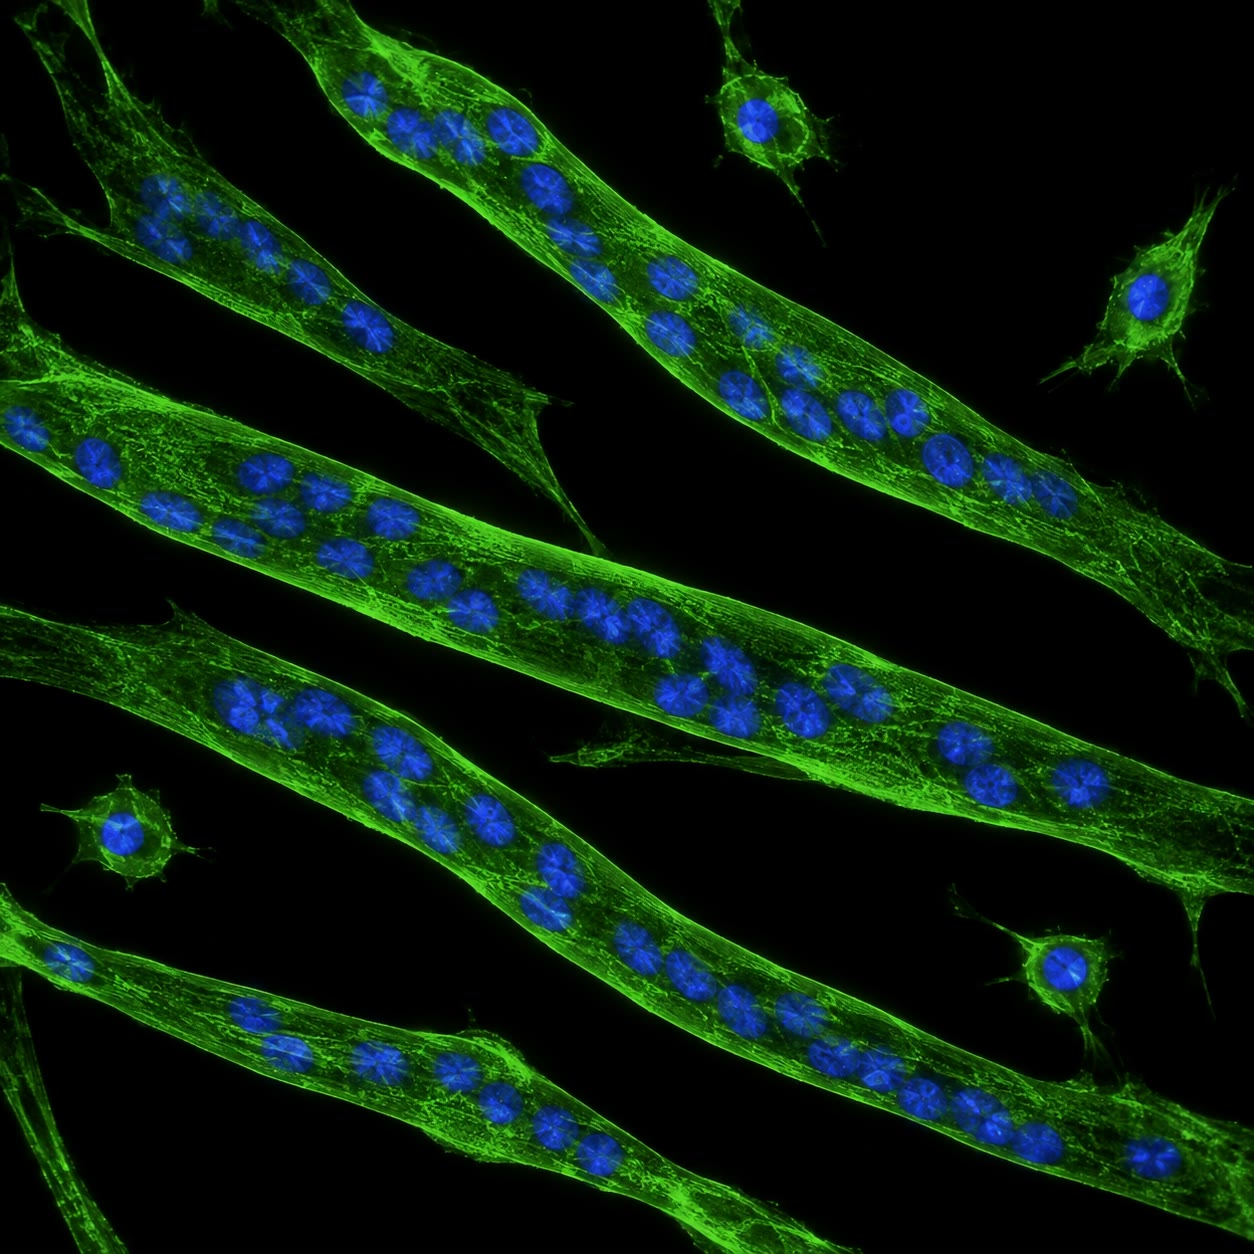
\includegraphics[width=0.44\linewidth]{images/book4/ai/b4-12-myotubes.jpg}\hspace{0.04\linewidth}
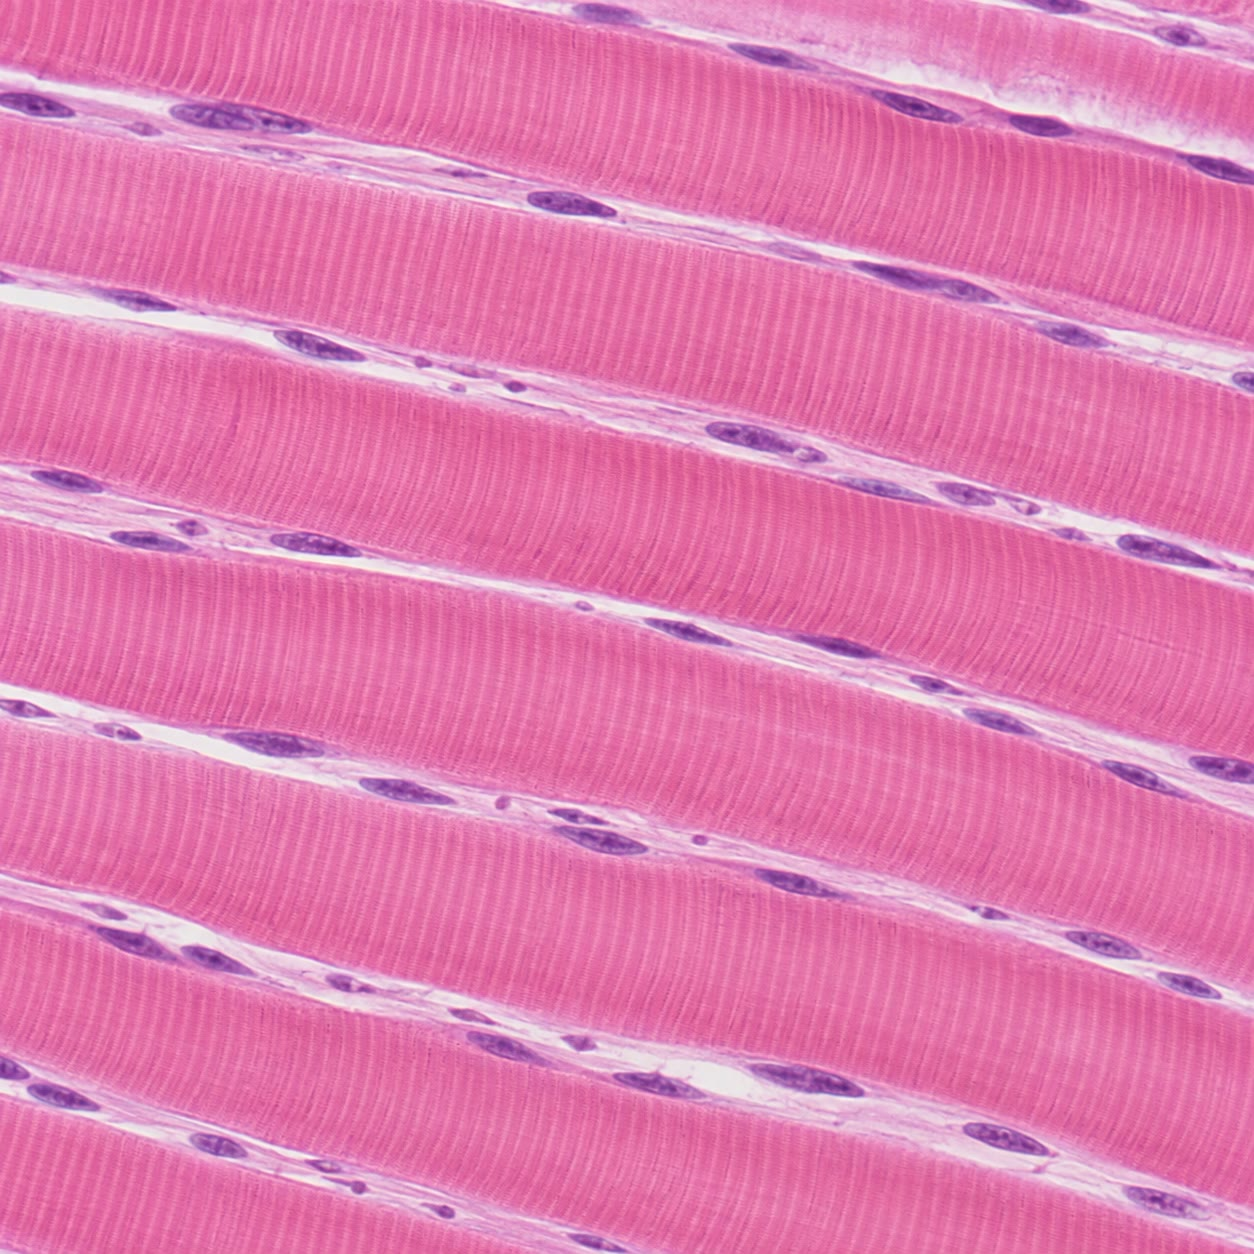
\includegraphics[width=0.44\linewidth]{images/book4/ai/b4-12-muscle-fibres.jpg}

{\small बाएँ: संवर्धन में \omterm{def:b2:cell-differentiation:myogenesis}{पेशीनलिकाएँ}, हर एक केंद्रकों की पंक्ति वाली
एक संलयित कोशिका, और उनके बग़ल अकेली \omterm{def:b2:cell-differentiation:myogenesis}{पेशीकोरक} जो अभी संलयित नहीं हुईं।
दाएँ: अनुदैर्घ्य दृश्य में परिपक्व तंतु, जिनकी आड़ी धारियाँ
दोहराती \omterm{def:b2:cell-differentiation:fibre}{सार्कोमियर} हैं और जिनके केंद्रक किनारे पर धकेल दिए गए हैं।}
\end{omfigure}

\begin{proposition}[MyoD: एक प्रमुख स्विच]\label{prop:b2:cell-differentiation:myod}
\index{प्रमुख नियामक!MyoD}
\omterm{def:b2:cell-differentiation:myogenesis}{MyoD} कुंडली-फंदा-कुंडली कुल का \omterm{prop:b2:cell-differentiation:transcriptional}{अनुलेखन कारक} है। वह,
किसी सर्वव्यापी साथी प्रोटीन के साथ द्विलक बनकर, पेशी-जीनों के नियामक
क्षेत्रों के छह-क्षारक अनुक्रम (E-बॉक्स, CANNTG) से
बँधता है, क्रोमैटिन खोलने वाले एंजाइम भर्ती करता है, और उन जीनों को चालू
कर देता है --- जिनमें मायोजेनिन के और स्वयं \omterm{def:b2:cell-differentiation:myogenesis}{MyoD} के जीन भी हैं, और
यों वह अवस्था टिकी रहती है। उसकी सक्रियता द्वार-नियंत्रित है: विभाजित
होते \omterm{def:b2:cell-differentiation:myogenesis}{पेशीकोरकों} में वृद्धि कारकों से प्रेरित कोई संदमक प्रोटीन (Id)
उस साथी को क़ब्ज़े में ले लेता है और \omterm{def:b2:cell-differentiation:myogenesis}{MyoD} को निठल्ला रखता है; और वृद्धि
कारक हटते ही Id लुप्त हो जाता है और \omterm{def:b2:cell-differentiation:myogenesis}{MyoD} काम करने लगता है। चूँकि \omterm{def:b2:cell-differentiation:myogenesis}{MyoD}
किसी तंतुकोरक, किसी वसाकोशिका या किसी तंत्रिका कोशिका पर पेशी-कार्यक्रम
थोपने को पर्याप्त है, इसलिए पेशी-नियति, एक अर्थ में, एक ही जीन गहरी है:
पेशी बनने की कठिनाई यह जानने में नहीं कि कैसे, बल्कि यह कहे जाने में है कि बनो।
\end{proposition}
\begin{proof}[प्रमाण-सामग्री]
डेविस, वाइनट्रॉब और लस्सार (1987) ने \omterm{def:b2:cell-differentiation:myogenesis}{पेशीकोरकों} से अलग की गई एक अकेली
cDNA संवर्धित तंतुकोरकों में डाली: वे तंतुकोरक
विभाजित होना बंद कर बैठे, \omterm{def:b2:cell-differentiation:myogenesis}{पेशीनलिकाओं} में संलयित हो गए और पेशी-प्रोटीन बनाने लगे।
उस जीन का नाम \omterm{def:b2:cell-differentiation:myogenesis}{MyoD} रखा गया। उसके सगे Myf5, मायोजेनिन और MRF4
समजातता से मिले; और जिस चूहे में \omterm{def:b2:cell-differentiation:myogenesis}{MyoD} तथा Myf5 दोनों न हों उसमें कोई
\omterm{def:b2:cell-differentiation:myogenesis}{पेशीकोरक} नहीं होते और कंकाल पेशी बिलकुल नहीं होती, जबकि जिस चूहे में
मायोजेनिन न हो उसके \omterm{def:b2:cell-differentiation:myogenesis}{पेशीकोरक} कभी संलयित नहीं होते।
\end{proof}

\begin{theorem}[स्वयं को बनाए रखता एक स्विच]\label{thm:b2:cell-differentiation:switch}
\index{द्विस्थायिता}\index{धन प्रतिपुष्टि!जीन}
मान लीजिए $m$ ऐसे किसी कारक की मात्रा है जो अपना ही जीन किसी
सहकारी (सिग्मॉइड) अनुक्रिया से सक्रिय करता है और $k$ दर से विघटित होता है:
\[
\frac{\mathrm{d}m}{\mathrm{d}t} = \frac{a\,m^{2}}{K^{2} + m^{2}} + b - k\,m,
\]
जिसमें $b$ कोई छोटा आधारी संश्लेषण है। $a$, $b$, $K$ और
$k$ के उपयुक्त मानों के लिए इस समीकरण की \emph{दो} स्थायी अवस्थाएँ हैं,
एक नीची $b/k$ के पास और एक ऊँची $a/k$ के पास, और उनके बीच एक अस्थिर
देहली: यानी वह कोशिका \emph{द्विस्थायी} है। कोई क्षणिक प्रेरक
संकेत जो $m$ को उस देहली से ऊपर धकेल दे उस कोशिका को ऊँची अवस्था में
भेज देता है, जहाँ वह संकेत हट जाने के बाद भी बनी रहती है; और उस देहली से
नीचे वह नीची अवस्था में लौट आती है। यह किसी प्रतिपुष्टि चक्र से गढ़ी गई
स्मृति है, और इसीलिए कोई कोशिका, एक बार प्रतिबद्ध हो जाने पर, विभाजनों
के आरपार और प्रेरक की अनुपस्थिति में भी प्रतिबद्ध बनी रहती है।
\end{theorem}
\begin{proof}
स्थायी अवस्थाएँ $k m = a m^{2}/(K^{2} + m^{2}) + b$ का पालन करती हैं।
दायाँ पक्ष $b$ से $a + b$ तक चढ़ता एक सिग्मॉइड है; और बायाँ
मूलबिंदु से होकर जाती $k$ ढाल की एक रेखा। $b/k < K$ के लिए और $k$ इतना
छोटा हो कि वह रेखा उस सिग्मॉइड के तीव्र भाग को काटे, तो दोनों
वक्र तीन बार कटते हैं: $m_{\text{निम्न}} \approx b/k$ पर, किसी
मध्यवर्ती $m_{\text{अ}}$ पर, और $m_{\text{उच्च}} \approx (a +
b)/k$ पर। स्थिरता: $m_{\text{निम्न}}$ से नीचे संश्लेषण क्षय से अधिक है और
$m$ चढ़ता है; $m_{\text{निम्न}}$ और $m_{\text{अ}}$ के बीच क्षय
संश्लेषण से अधिक है और $m$ गिरकर लौट आता है; $m_{\text{अ}}$ और
$m_{\text{उच्च}}$ के बीच संश्लेषण क्षय से अधिक है और $m$ चढ़कर
$m_{\text{उच्च}}$ तक जाता है; और उससे ऊपर $m$ गिरकर $m_{\text{उच्च}}$ पर लौट आता है।
इसलिए बाहरी दोनों स्थिर हैं, और बीच वाली अस्थिर तथा
वही देहली है।
\end{proof}

\begin{omfigure}
\begin{tikzpicture}
\begin{axis}[
  width=0.74\linewidth, height=5.8cm,
  axis x line=bottom, axis y line=left,
  xmin=0, xmax=4, ymin=0, ymax=1.3,
  xlabel={कारक का स्तर $m$ (सापेक्ष)}, ylabel={दर},
  xlabel style={font=\small, at={(axis description cs:0.5,-0.12)}, anchor=north},
  ylabel style={font=\small},
  tick label style={font=\small}, xtick={0,1,2,3,4}, ytick={0,0.5,1},
  legend style={font=\scriptsize, at={(0.03,0.97)}, anchor=north west, draw=none},
  clip=false,
]
\addplot[very thick, omDef, domain=0:4, samples=100] {x^2/(1+x^2) + 0.02};
\addlegendentry{संश्लेषण: $a m^2/(K^2 + m^2) + b$}
\addplot[very thick, omThm, domain=0:3.2, samples=2] {0.4*x};
\addlegendentry{विघटन: $k m$}
\fill[omDef] (axis cs:0.055,0.022) circle (2pt); \draw[gray] (axis cs:0.08,0.04) -- (axis cs:0.33,0.42); \node[font=\scriptsize, anchor=west] at (axis cs:0.35,0.45) {बंद};
\draw[gray, thick] (axis cs:0.41,0.164) circle (2pt); \node[font=\scriptsize, anchor=west] at (axis cs:0.55,0.10) {देहली};
\fill[omDef] (axis cs:2.1,0.84) circle (2pt); \node[font=\scriptsize, anchor=north] at (axis cs:2.1,0.78) {चालू};
\end{axis}
\end{tikzpicture}

{\small एक द्विस्थायी स्विच ($a = 1$, $K = 1$, $b = 0.02$, $k = 0.4$)।
संश्लेषण (सिग्मॉइड) और विघटन (रेखा) तीन बार कटते हैं: दो
स्थायी अवस्थाएँ, बंद और चालू, और उनके बीच एक अस्थिर देहली।
जो संकेत $m$ को उस देहली के पार उठा दे वह उस कोशिका को स्थायी रूप से
चालू अवस्था पर प्रतिबद्ध कर देता है।}
\end{omfigure}

\section{तैयार कोशिका}

\begin{definition}[पेशी तंतु]\label{def:b2:cell-differentiation:fibre}
\index{सार्कोमियर}\index{पेशीतंतुक}\index{पेशीद्रव्यी जालिका}\index{T नलिका}
कोई कंकाल \omterm{def:b2:cell-differentiation:myogenesis}{पेशी तंतु} \qtyrange{10}{100}{\micro m}
चौड़ा और दसियों सेंटीमीटर तक लंबा बेलन है, जो
\emph{पेशीकला} से घिरा है और जिसके सैकड़ों केंद्रक उसी के ठीक नीचे हैं।
उसका भीतरी भाग समांतर \emph{पेशीतंतुकों} से भरा है, और हर एक
\qty{2.5}{\micro m} लंबी \emph{सार्कोमियरों} की शृंखला है: दो Z चक्रिकाओं
के बीच, Z चक्रिकाओं पर टिके ऐक्टिन के पतले तंतु (ट्रोपोमायोसिन और
ट्रोपोनिन सहित) केंद्र पर थामे मायोसिन के मोटे तंतुओं के बीच घुस जाते
हैं, और उस अतिव्यापन का प्रतिरूप ही वे धारियाँ देता है। हर
पेशीतंतुक के चारों ओर \emph{पेशीद्रव्यी जालिका} की एक जाली कैल्सियम
सँजोए रखती है; और \emph{अनुप्रस्थ नलिकाएँ}, जो पेशीकला के अंतर्वलन हैं,
पेशीतंतुकों के बीच चलती हैं और उस विद्युत संकेत को सतह से भीतर तक ले
जाती हैं। सूत्रकणिकाएँ बीच की जगहें भर देती हैं, और
कोशिकाद्रव्य में ग्लाइकोजन, क्रिएटिन फ़ॉस्फ़ेट और, लाल तंतुओं में,
मायोग्लोबिन होता है। वह कोशिका एक ही काम के लिए बनी है --- आज्ञा पर
छोटा होने के लिए --- और उस आज्ञा का साज-सामान
\cref{ch:b2:muscle-movement} है।
\end{definition}

\begin{omfigure}
\begin{tikzpicture}[every node/.style={font=\scriptsize}]
  % a stretch of myofibril with two sarcomeres
  \foreach \s in {0,4.4} {
    \begin{scope}[xshift=\s cm]
      \draw[very thick, omThm] (0,-1.1) -- (0,1.1);
      \foreach \y in {-0.9,-0.5,-0.1,0.3,0.7} { \draw[thick, omDef] (0,\y) -- (1.6,\y); \draw[thick, omDef] (4.4,\y) -- (2.8,\y); }
      \foreach \y in {-0.7,-0.3,0.1,0.5,0.9} { \draw[line width=3pt, omExo!80!black] (1.0,\y) -- (3.4,\y); }
      \draw[gray] (2.2,-1.1) -- (2.2,1.1);
    \end{scope}
  }
  \draw[very thick, omThm] (8.8,-1.1) -- (8.8,1.1);
  \node[omThm, below] at (0,-1.15) {Z चक्रिका};
  \node[omThm, below] at (4.4,-1.15) {Z चक्रिका};
  \node[omThm, below] at (8.8,-1.15) {Z चक्रिका};
  \node[omDef, above] at (0.8,1.15) {पतले तंतु (ऐक्टिन)};
  \node[omExo!80!black, above] at (6.6,1.15) {मोटे तंतु (मायोसिन)};
  \node[gray, below] at (2.2,-1.15) {M रेखा};
  \draw[<->] (0,1.9) -- (4.4,1.9); \node[above] at (2.2,1.9) {एक सार्कोमियर, \qty{2.5}{\micro m}};
  \draw[<->] (5.4,-1.6) -- (7.8,-1.6); \node[below] at (6.6,-1.6) {A पट्टी (गहरी)};
  \draw[<->] (7.8,-1.6) -- (9.8,-1.6); \node[below] at (8.8,-1.6) {I पट्टी (हलकी)};
\end{tikzpicture}

{\small किसी \omterm{def:b2:cell-differentiation:fibre}{पेशीतंतुक} की दो \omterm{def:b2:cell-differentiation:fibre}{सार्कोमियर}: Z चक्रिकाओं पर टिके पतले
ऐक्टिन तंतु M रेखा पर केंद्रित मोटे मायोसिन तंतुओं के बीच घुस जाते हैं।
उस अतिव्यापन से धारियों की गहरी A पट्टी और हलकी I पट्टी बनती हैं।}
\end{omfigure}

\begin{proposition}[तंतु के प्रकार]\label{prop:b2:cell-differentiation:types}
\index{पेशी तंतु के प्रकार}
कोई पेशी तंतु-प्रकारों का मिश्रण है, जो कुछ हद तक \omterm{def:b2:cell-differentiation:myogenesis}{पेशीकोरक}
वंशक्रम से और कुछ हद तक उस तंतु को तंत्रिकित करती तंत्रिका से तय होता है।
\emph{मंद ऑक्सीकारी} (प्रकार I) तंतुओं में मंद मायोसिन, बहुत-सी
सूत्रकणिकाएँ तथा केशिकाएँ, और मायोग्लोबिन होते हैं --- यानी लाल, अथक,
और मुद्रा तथा सहनशक्ति के लिए बने। \emph{तीव्र ग्लाइकोलीय} (प्रकार IIx)
तंतुओं में तीव्र मायोसिन, थोड़ी सूत्रकणिकाएँ, बहुत ग्लाइकोजन होता है ---
यानी सफ़ेद, बलवान, और मिनट भर में थक जाने वाले। \emph{तीव्र ऑक्सीकारी}
(प्रकार IIa) तंतु बीच में पड़ते हैं। किसी धावक की पिंडली अधिकतर तीव्र
तंतुओं की है, किसी मैराथन धावक की अधिकतर मंद, और वे अनुपात वंशागत हैं;
पर वह प्रकार नियत नहीं है: किसी तीव्र पेशी को किसी मंद तंत्रिका से
आड़े-तिरछे तंत्रिकित करना, या महीनों का सहनशक्ति प्रशिक्षण, तंतुओं को
मंद प्रकार की ओर बदल देता है, क्योंकि तंत्रिका-आवेगों का प्रतिरूप
मायोसिन समरूपों के और सूत्रकणिका-जनन के जीन चालू-बंद करता है।
कोई विभेदित कोशिका \omterm{def:b2:cell-differentiation:myogenesis}{पेशी तंतु} के रूप में अपनी पहचान बनाए रखती है
और फिर भी उपयोग के उत्तर में अपना कार्यक्रम संशोधित करती है।
\end{proposition}

\begin{example}[वृद्धि और मरम्मत]\label{ex:b2:cell-differentiation:satellite}
वयस्क में कोई \omterm{def:b2:cell-differentiation:myogenesis}{पेशी तंतु} जोड़कर नहीं बल्कि उन्हें बड़ा करके बढ़ती है:
प्रशिक्षण हर तंतु में \omterm{def:b2:cell-differentiation:fibre}{पेशीतंतुक} जोड़ता है, और \emph{उपग्रही
कोशिकाएँ} उसमें संलयित होकर वे अतिरिक्त केंद्रक जुटाती हैं जो किसी बड़े
कोशिकाद्रव्य को चाहिए। चोट के बाद वही कोशिकाएँ विभाजित होती हैं, फिर से
\omterm{def:b2:cell-differentiation:myogenesis}{MyoD} अभिव्यक्त करती हैं, संलयित होती हैं और क्षतिग्रस्त खंड को
सप्ताहों में फिर गढ़ देती हैं --- यानी वही भ्रूणीय कार्यक्रम वयस्क में
फिर चलाया जाता है। पेशीय दुष्पोषण में उन तंतुओं में
डिस्ट्रोफ़िन नहीं होता, यानी वह प्रोटीन जो \omterm{def:b2:cell-differentiation:fibre}{पेशीतंतुकों} को
झिल्ली से बाँधता है, और वे संकुचन में फट जाते हैं; और उपग्रही कोशिकाएँ
उनकी बार-बार मरम्मत करती हैं जब तक, वर्षों बाद, वह भंडार चुक नहीं जाता
और उस पेशी का स्थान तंतुमय ऊतक नहीं ले लेता।
\end{example}

\begin{omfigure}
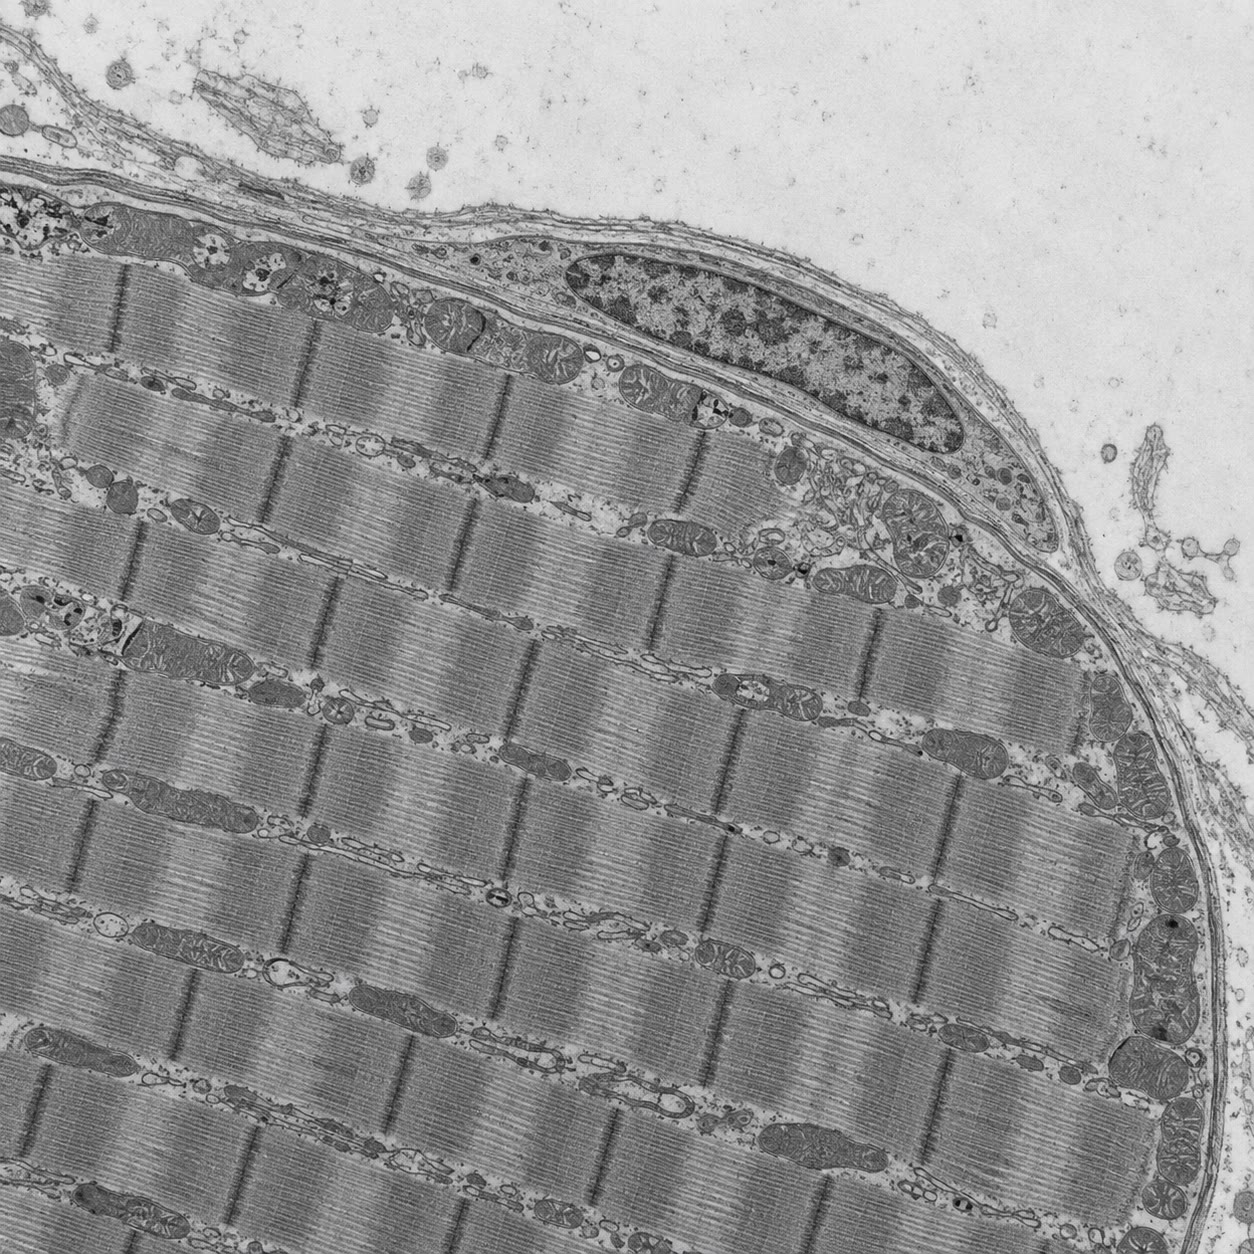
\includegraphics[width=0.42\linewidth]{images/book4/ai/b4-12-satellite-cell-tem.jpg}

{\small इलेक्ट्रॉन सूक्ष्मदर्शी के नीचे एक उपग्रही कोशिका: किसी
\omterm{def:b2:cell-differentiation:myogenesis}{पेशी तंतु} की झिल्ली और उसकी आधार पटलिका के बीच दबी एक छोटी
एककेंद्रकी कोशिका --- यानी उस तंतु का पेशीकोरक-भंडार।}
\end{omfigure}

\section{अभ्यास}

\begin{exercise}[$\star$]\label{exo:b2:cell-differentiation:1}
\omterm{def:b2:cell-differentiation:differentiation}{विभेदन}, निर्धारण और \omterm{def:b2:cell-differentiation:differentiation}{शक्तता} की परिभाषा दीजिए, और
युग्मनज, \omterm{def:b2:mammal-reproduction:implantation}{अंतःकोशिका पिंड} की कोई कोशिका, कोई उपग्रही कोशिका तथा कोई \omterm{def:b2:cell-differentiation:myogenesis}{पेशी तंतु}
\omterm{def:b2:cell-differentiation:differentiation}{शक्तता} की मापनी पर रखिए।
\end{exercise}

\begin{exercise}[$\star$]\label{exo:b2:cell-differentiation:2}
कायखंड की कोशिका से \omterm{def:b2:cell-differentiation:myogenesis}{पेशी तंतु} तक पेशीजनन के चरण बताइए, और
हर एक पर अभिव्यक्त होता \omterm{prop:b2:cell-differentiation:transcriptional}{अनुलेखन कारक}।
\end{exercise}

\begin{exercise}[$\star$]\label{exo:b2:cell-differentiation:3}
गर्डन के केंद्रक-प्रत्यारोपण ने क्या दिखाया, और क्या नहीं दिखाया?
\end{exercise}

\begin{exercise}[$\star$]\label{exo:b2:cell-differentiation:4}
किसी \omterm{def:b2:cell-differentiation:fibre}{सार्कोमियर} के भाग बताइए और कहिए कि तंतु के छोटे होने पर
कौन-से चलते हैं और कौन-से नहीं।
\end{exercise}

\begin{exercise}[$\star\star$]\label{exo:b2:cell-differentiation:5}
\qty{20}{cm} लंबे किसी तंतु में \qty{2.5}{\micro m} की \omterm{def:b2:cell-differentiation:fibre}{सार्कोमियर} हैं और
उसकी लंबाई के हर \qty{25}{\micro m} पर एक केंद्रक। शृंखला में कितनी
\omterm{def:b2:cell-differentiation:fibre}{सार्कोमियर}, और कितने केंद्रक? उसे बनाने के लिए कितने \omterm{def:b2:cell-differentiation:myogenesis}{पेशीकोरक} संलयित
हुए?
\end{exercise}

\begin{exercise}[$\star\star$]\label{exo:b2:cell-differentiation:6}
संदमक Id से समझाइए कि FGF की उपस्थिति में \omterm{def:b2:cell-differentiation:myogenesis}{पेशीकोरक} संलयित क्यों नहीं
होते, और भविष्यवाणी कीजिए कि जिन \omterm{def:b2:cell-differentiation:myogenesis}{पेशीकोरकों} को Id लगातार
बनाने को गढ़ा गया हो उनका क्या होता है।
\end{exercise}

\begin{exercise}[$\star\star$]\label{exo:b2:cell-differentiation:7}
स्विच मॉडल में $a = 1$, $K = 1$, $b = 0.02$ और $k = 0.4$ के साथ,
प्रतिस्थापन से जाँचिए कि $m = 2.1$ किसी स्थायी अवस्था के पास है,
नीची स्थायी अवस्था लगभग ढूँढ़िए, और बताइए कि जिस कोशिका का $m$ थोड़ी देर
के लिए $1$ तक चढ़ाकर फिर छोड़ दिया जाए उसका क्या होता है।
\end{exercise}

\begin{exercise}[$\star\star$]\label{exo:b2:cell-differentiation:8}
उसी मॉडल में $k$ बढ़ाकर $0.6$ किया जाता है (यानी वह कारक तेज़ी से
विघटित होता है)। आलेख से या संख्याओं से दिखाइए कि ऊँची अवस्था
लुप्त हो जाती है। यह ऐसी किसी कोशिका के लिए क्या भविष्यवाणी करता है
जिसमें \omterm{def:b2:cell-differentiation:myogenesis}{MyoD} अस्थिर कर दी गई हो?
\end{exercise}

\begin{exercise}[$\star\star$]\label{exo:b2:cell-differentiation:9}
ऐसे किसी चूहे के \omterm{def:b2:meiosis-heredity:vocabulary}{लक्षण-प्ररूप} की भविष्यवाणी कीजिए जिसमें (क) \omterm{def:b2:cell-differentiation:myogenesis}{MyoD} और
Myf5 दोनों न हों, (ख) केवल मायोजेनिन न हो, (ग) केवल \omterm{def:b2:cell-differentiation:myogenesis}{MyoD} न हो। (ग) लगभग सामान्य क्यों है?
\end{exercise}

\begin{exercise}[$\star\star\star$]\label{exo:b2:cell-differentiation:10}
\omterm{def:b2:cell-differentiation:myogenesis}{MyoD} से अभिरंजित कोई तंतुकोरक \omterm{def:b2:cell-differentiation:myogenesis}{पेशीनलिका} बन जाता है; पर \omterm{def:b2:cell-differentiation:myogenesis}{MyoD} से
अभिरंजित कोई यकृत कोशिका नहीं बनती। क्रोमैटिन और \omterm{def:b2:vertebrate-development:induction}{सक्षमता} को
जोड़ते हुए कोई स्पष्टीकरण सुझाइए, और उसे परखने का कोई प्रयोग।
\end{exercise}

\begin{exercise}[$\star\star\star$]\label{exo:b2:cell-differentiation:11}
सहनशक्ति प्रशिक्षण तीव्र तंतुओं को उनका जीनोम बदले बिना मंद तंतुओं की
ओर बदल देता है। जीन-अभिव्यक्ति के पदों में समझाइए कि तंत्रिका के
स्फुरण-प्रतिरूप से यह कैसे हो सकता है, और वे तंतु फिर भी कंकाल पेशी क्यों
बने रहते हैं और कभी, मान लीजिए, उपास्थि क्यों नहीं बनते।
\end{exercise}

\begin{exercise}[$\star\star\star$]\label{exo:b2:cell-differentiation:12}
``कोई विभेदित कोशिका याद रखती है कि वह क्या है, किसी परिपथ से, किसी
\omterm{def:b2:genome-diversification:mutation}{उत्परिवर्तन} से नहीं।'' द्विस्थायी स्विच, क्रोमैटिन, और इस तथ्य के साथ
इस पर विचार कीजिए कि गर्डन तथा यामानाका के पुनर्बिठान संभव तो हैं पर
अदक्ष।
\end{exercise}

\section{समस्या: एक पेशी गढ़ी और फिर गढ़ी गई}

\begin{problem}[{सप्तांत समस्या --- किसी पेशी का कायखंड से तंतु तक और
चोट के आरपार पीछा: पेशीकोरकों, संलयनों तथा केंद्रकों की संख्याएँ,
द्विस्थायी स्विच का विश्लेषण, किसी मरम्मत का समय, और प्रशिक्षण की
गणना, और अंत तंतु की केंद्रक-गणना, स्विच की देहली तथा मरम्मत के काल पर}]
\label{pb:b2:cell-differentiation:1}
किसी वयस्क की जाँघ-पेशी में \num{500000} तंतु हैं, हर एक
\qty{20}{cm} लंबा और \qty{60}{\micro m} व्यास का, और लंबाई के हर
\qty{25}{\micro m} पर एक केंद्रक; \omterm{def:b2:cell-differentiation:fibre}{सार्कोमियर}
\qty{2.5}{\micro m} की हैं। भ्रूणीय \omterm{def:b2:cell-differentiation:myogenesis}{पेशीकोरक}, FGF रहते,
हर \qty{12}{h} पर विभाजित होते हैं। स्विच मॉडल: $a = 1$, $K = 1$, $b = 0.02$, $k
= 0.4$। हर तंतु की \qty{10}{\%} लंबाई नष्ट करती किसी चोट के बाद,
घायल खंड की उपग्रही कोशिकाएँ (तंतु के प्रति मिलिमीटर \num{4}) कुछ समय
हर \qty{18}{h} पर विभाजित होती हैं, फिर संलयित हो जाती हैं।

\medskip
\noindent\textbf{भाग I --- तंतु।}
\begin{enumerate}
  \item एक तंतु में शृंखला में \omterm{def:b2:cell-differentiation:fibre}{सार्कोमियरों} की संख्या और
        केंद्रकों की संख्या निकालिए।
  \item एक तंतु बनाने को कितने \omterm{def:b2:cell-differentiation:myogenesis}{पेशीकोरक} संलयित हुए? और पूरी पेशी के लिए?
  \item एक तंतु का और उस पेशी का आयतन (लिटर में)
        निकालिए।
  \item एक केंद्रक जितना कोशिकाद्रव्यी आयतन सँभालता है उसका आकलन कीजिए, और
        \qty{2000}{\micro m^3} की किसी साधारण कोशिका से तुलना कीजिए।
  \item किसी परिपक्व तंतु के केंद्रक उसकी परिधि पर क्यों पड़े होते हैं?
  \item उस पेशी के \omterm{def:b2:cell-differentiation:myogenesis}{पेशीकोरक} \num{2000} कायखंड-कोशिकाओं से उतरे थे।
        प्रश्न 2 की संख्या तक पहुँचने को उन्हें कितने दुगुनेपन चाहिए थे,
        और कितने दिन?
\end{enumerate}

\medskip
\noindent\textbf{भाग II --- स्विच।}
\begin{enumerate}[resume]
  \item स्थायी-अवस्था की शर्त लिखिए और दिखाइए कि $m \approx
        0.055$ उसका पालन करता है।
  \item दिखाइए कि $m \approx 2.1$ भी उसका पालन करता है।
  \item दिखाइए कि $m = 0.41$ के पास एक तीसरा हल है, और
        दोनों ओर $\mathrm{d}m/\mathrm{d}t$ के चिह्नों से
        समझाइए कि वह अस्थिर है।
  \item प्रेरक की एक स्पंद $m$ को $0.6$ तक चढ़ा देती है; और दूसरी $0.3$ तक।
        हर कोशिका की नियति क्या है?
  \item कोई \omterm{def:b2:genome-diversification:mutation}{उत्परिवर्तन} आधारी संश्लेषण $b$ को बढ़ाकर $0.4$ कर देता है।
        दिखाइए कि नीची अवस्था लुप्त हो जाती है। वह कोशिका क्या करती है?
  \item समझाइए कि यह मॉडल कोशिका-विभाजन के आरपार प्रतिबद्धता के बचे
        रहने का क्या लेखा देता है, और हर विभाजन पर $m$ के बारे में क्या सच होना चाहिए।
\end{enumerate}

\medskip
\noindent\textbf{भाग III --- मरम्मत।}
\begin{enumerate}[resume]
  \item एक तंतु कितनी उपग्रही कोशिकाएँ ढोता है, और उस चोट के बाद कितने
        केंद्रक बदलने पड़ते हैं?
  \item उन्हें जुटाने के लिए उपग्रही कोशिकाओं को कितने दुगुनेपन से
        गुज़रना पड़ता है, और उसमें कितना समय लगता है?
  \item मरम्मत के लिए प्रेक्षित दो से तीन सप्ताह से तुलना कीजिए, और
        बताइए कि उस काल में और क्या-क्या सम्मिलित है।
  \item उपग्रही कोशिकाओं को संलयित होने से पहले \omterm{def:b2:cell-differentiation:myogenesis}{MyoD} फिर क्यों
        अभिव्यक्त करनी पड़ती है, और उन्हें पहले विभाजित होना क्यों बंद करना पड़ता है?
  \item मरम्मत का हर दौर कुछ उपग्रही कोशिकाएँ चुका देता है। यदि वह
        भंडार प्रति चोट \qty{5}{\%} घटे, तो उसके आधा होने से पहले कितनी
        चोटें?
  \item ऐसी बीस चोटों के बाद प्रति तंतु कितनी उपग्रही कोशिकाएँ बचती हैं?
  \item समझाइए कि जिस दुष्पोषी पेशी के तंतु हर संकुचन पर फटते हैं उसका
        स्थान वर्षों बाद तंतुमय ऊतक क्यों ले लेता है।
\end{enumerate}

\medskip
\noindent\textbf{भाग IV --- प्रशिक्षण।}
\begin{enumerate}[resume]
  \item प्रशिक्षण हर तंतु को मोटा करके \qty{80}{\micro m} कर देता है।
        उस तंतु का आयतन कितने गुना बढ़ता है, और यदि प्रश्न 4 का अनुपात
        बनाए रखा जाए तो उपग्रही कोशिकाओं को कितने अतिरिक्त
        केंद्रक जुटाने पड़ते हैं?
  \item उस पेशी का नया आयतन निकालिए।
  \item सहनशक्ति प्रशिक्षण तीव्र तंतुओं का \qty{30}{\%} मंद तंतुओं में
        बदल देता है। उन तंतुओं में क्या बदला है और क्या नहीं?
  \item इस तथ्य से समझाइए कि तंतु विभाजित नहीं होते, कि कोई वयस्क \omterm{def:b2:cell-differentiation:myogenesis}{पेशी
        तंतु} जोड़कर नहीं बल्कि तंतुओं की वृद्धि से क्यों बड़ी होती है।
  \item कोई औषधि उपग्रही कोशिकाओं का संलयन रोक देती है। प्रशिक्षण के
        और चोट के प्रति उस पेशी की अनुक्रिया की भविष्यवाणी कीजिए।
  \item परिणाम बताइए: तंतु की केंद्रक-गणना, स्विच की देहली,
        और मरम्मत के केंद्रक जुटाने में उपग्रही कोशिकाओं को लगने वाला काल।
\end{enumerate}
\end{problem}
